\renewcommand{\chapid}{app}

\chapter*{Appendices \chaplabel{app}}
\addcontentsline{toc}{chapter}{Appendices}
\setcounter{chapter}{-1}
\setcounter{section}{0}
\setcounter{subsection}{0}
% \setcounter{figure}{0}
% \setcounter{equation}{0}
\counterwithin*{equation}{section}
\counterwithin*{figure}{section}
\counterwithin*{table}{section}
\renewcommand{\thefigure}{\thesection.\arabic{figure}}
\renewcommand{\thetable}{\thesection.\arabic{table}}
\renewcommand{\theequation}{\thesection.\arabic{equation}}
\renewcommand{\thesection}{\Alph{section}}
\addtocontents{toc}{\protect\setcounter{tocdepth}{0}}


%This \paper\ represents joint work with [people] published in [place] as [citation].

%\section{Chapter abstract}
%
%[probably the paper abstract]
%
%\section{Introduction}
%
%[probably the paper intro, and then all the other sections from the paper]


\section{Primer on the Kullback-Leibler Divergence}
\appendices{Appendix to \chap{qp}: A Primer on the Kullback-Leibler Divergence}
\label{app:kld}

We develop some intuition for the Kullback-Leibler Divergence by contrasting it 
with the familiar metric of the root-mean-square error (RMSE)
\begin{align}
\eqlabel{eq:rmse}
\mathrm{RMSE} &= \sqrt{\int (P(z) - \hat{P}(z))^{2} dz}.
\end{align}
Consider the simple example of a Gaussian $P(z) = \mathcal{N}(\mu_{0}, 
\sigma_{0}^{2})$ being approximated by a Gaussian $\hat{P}(z) = 
\mathcal{N}(\mu, \sigma^{2})$, whose KLD is
\begin{align}
\eqlabel{eq:gaussian}
\mathrm{KLD} &= 
\frac{1}{2}\left(\log\left[\frac{\sigma^{2}}{\sigma_{0}^{2}}\right] + 
\frac{\sigma_{0}^{2}}{\sigma^{2}} + \frac{(\mu-\mu_{0})^{2}}{\sigma^{2}} - 
1\right)
\end{align}
To get a sense of the units of information, we can calculate the KLD and RMSE 
in some limiting cases.
If $\sigma=\sigma_{0}$ but $\mu=\mu_{0}+1$, we obtain 
$\mathrm{KLD}=\frac{1}{2}$ nat -- if the mean of the approximation is wrong by 
an additive factor of $\sigma$, half a nat of information is lost.
If $\mu=\mu_{0}$ but $\sigma=\sqrt{2\pi}\sigma_{0}$, we find 
$\mathrm{KLD}\approx\frac{1}{2}$ nat -- half a nat of information is also lost 
if the variance of the approximation is off by a multiplicative factor of 
$2\pi$.

We can use the KLD to identify notions of imprecision and inaccuracy.
Intuitively, precision must be related to how close $\sigma$ is to $\sigma_{0}$ 
and accuracy must be related to how close $\mu$ is to $\mu_{0}$.

\begin{figure}
	\begin{center}
		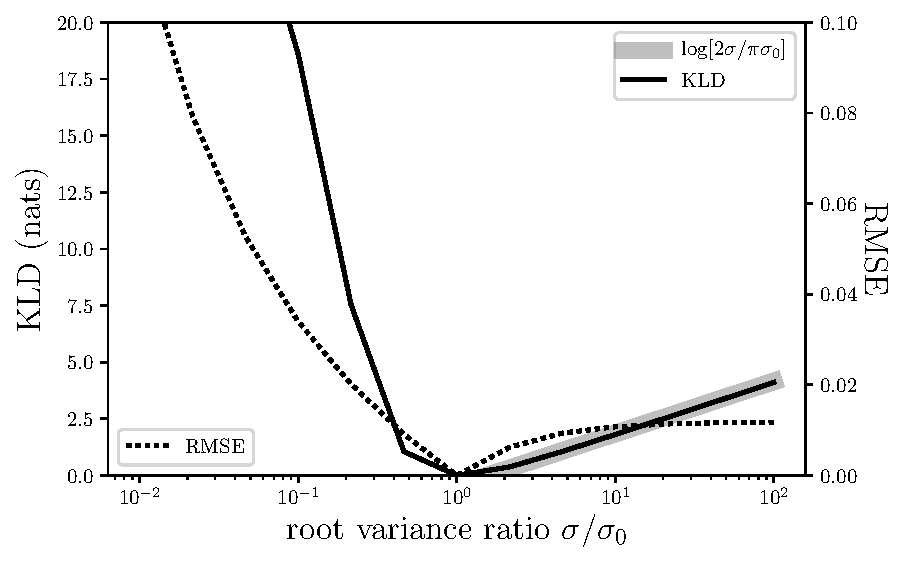
\includegraphics[width=0.74\columnwidth]{figures/qp/precision.pdf}
		\caption[The KLD and RMSE as a function of the root variance ratio $r$ for 
		a simple Gaussian example]
		{The KLD and RMSE as a function of the root variance ratio $r$ for 
			a simple Gaussian example.
			The KLD (solid line) rises sharply at $\sigma<\sigma_{0}$ and is 
			proportional to the log of the inverse precision $r$ for $\sigma>\sigma_{0}$, 
			behavior that is qualitatively similar to that of the RMSE (dotted line).
			\figlabel{fig:precision}}
	\end{center}
\end{figure}

If $\mu\approx\mu_{0}$, we can say $\mathrm{KLD}\sim\log[r] + \frac{1}{2}r^{-2} 
- \frac{1}{2}$ where $r^{-1}\equiv\frac{\sigma_{0}}{\sigma}$ is a measure of 
\textit{precision}, whose behavior is illustrated in 
\Fig{fig:precision}, alongside that of the RMSE.  We observe that an 
overestimated variance increases the KLD as the log of the square root of the 
ratio of the estimated variance to the true variance.

\begin{figure}
	\begin{center}
		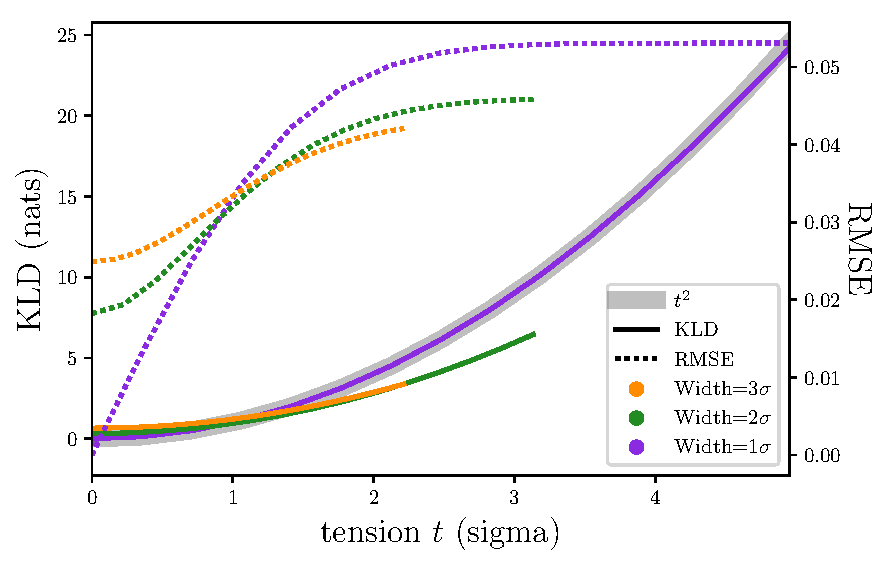
\includegraphics[width=0.74\columnwidth]{figures/qp/tension.pdf}
		\caption[The KLD and RMSE as a function of the tension $t$ for a simple 
		Gaussian example]
		{The KLD and RMSE as a function of the tension $t$ for a simple 
			Gaussian example.
			The KLD (solid lines) is equal to the square of the tension $t$, with a 
			small offset when $r\neq1$, whereas the RMSE (dotted lines) is relatively 
			insensitive to tension past a certain point but more sensitive to $r\neq1$.
			\figlabel{fig:tension}}
	\end{center}
\end{figure}

When $\sigma\approx\sigma_{0}$, $\mathrm{KLD}\sim t^{2}$ in terms of the 
\textit{tension} $t\equiv\frac{(\mu-\mu_{0})^{2}}{\sigma^{2}}$, whose 
concordance is illustrated in \Fig{fig:tension}.
There is some limiting tension $t_{\mathrm{lim}}\approx2$ below which the RMSE 
is more sensitive than the KLD and above which the KLD is more sensitive than 
the RMSE.
This behavior hints at the KLD's reputation for sensitivity to the tails of the 
reference distribution.
The notion of tension may be more important for cosmological applications of 
\pz s, indicating the KLD may be a more appropriate metric for coarser 
approximations and the RMSE may be a more appropriate metric for less coarse 
approximations.


\section{Evaluation of Supplemental Metrics of \Pzpdf s}
\appendices{Appendix to \chap{pzdc1}: Evaluation of Supplemental Metrics of \Pzpdf s}
\label{app:pzdc1}

\subsection{Evaluation of the redshift distribution}
%\appendices{Evaluation of the redshift distribution}
\label{sec:moments}
%(Alex Malz)

Perhaps the most popular application of \pzpdf s is the estimation of the overall redshift distribution $N(z)$, a quantity that enters some cosmological calculations and the true value of which is known for the DC1 data set and will be denoted as $\tilde{N}(z)$.
In terms of the prior information provided to each method, the true redshift distribution satisfies the tautology $\tilde{N}(z) = p(z \vert I_{D})$ due to our experimental set-up; 
because the DC1 training and template sets are representative and complete, $I_{D}$ represents a prior that is also equal to the truth.
In this ideal case of complete and representative prior information, the method that would give the best approximation to $\hat{N}(z)$ would be one that neglects all the information contained in the photometry $\{d_{i}\}_{N_{tot}}$ and gives every galaxy the same \pzpdf\ $\hat{p}_{i}(z) = \tilde{N}(z)$ for all $i$; 
the inclusion of any information from the photometry would only introduce noise to the optimal result of returning the prior.
This is the exact estimator, \trainz, that we have described in Section~\ref{pzdc1:sect:sec:trainz}, and which will serve as an experimental control.

\subsubsection{Metrics of the stacked estimator of the redshift distribution}
%\appendices{Metrics of the stacked estimator of the redshift distribution}
\label{sec:stackedmetrics}

% Though alternatives exist \citep{malz_cosmological_2018}, 
``Stacking'' according to
\begin{equation}
\eqlabel{eq:stacked}
\hat{N}^{H}(z) \equiv \frac{1}{N_{tot}}\ \sum_{i}^{N_{tot}}\ \hat{p}^{H}_{i}(z)
\end{equation}
is the most widely used method for obtaining $\hat{N}^{H}(z)$ as an estimator of the redshift distribution from \pzpdf s derived by a method $H$.
While the stacked estimator of the redshift distribution violates the mathematical definition of statistical independence and is thus not formally correct\footnote{\Chap{chippr} shows how the stacking procedure can lead to bias in the estimate of $N(z)$ and presents a principled alternative to this commonly employed method.  See \url{https://github.com/aimalz/chippr} for details.}, we use it as a basis for comparison of \pzpdf\ methods under the untested assumption that the response of our metrics of $\hat{N}^{H}(z)$ will be analogous to the same metrics applied to a principled estimator of the redshift distribution.
% Though we do not endorse the use of the stacked estimator of the redshift distribution, we use it under the untested assumption that the response of our metrics of $\hat{N}^{H}(z)$ will be analogous to the same metrics applied to a principled estimator of the redshift distribution.

As $N(z)$ is itself a univariate PDF, we apply the metrics of the previous sections to it as well.
We additionaly calculate the first three moments
\begin{equation}
\eqlabel{eq:moment}
\langle z^{m}\rangle \equiv \int_{-\infty}^{\infty} z^{m} N(z) dz
\end{equation}
of the estimated redshift distribution $\hat{N}^{H}(z)$ for each code and compare them to the moments of the true redshift distribution $\tilde{N}(z)$.
Under the assumption that the stacked estimator is unbiased, a superior method minimizes the difference between the true and estimated moments.

\subsubsection{Performance on the stacked estimator of the redshift distribution}
%\appendices{Performance on the stacked estimator of the redshift distribution}
\label{sec:stackedmetrics_results}

\Fig{fig:nz} shows the stacked estimator $\hat{N}(z)$ of the redshift distribution for each code compared to the true redshift distribution $\tilde{N}(z)$, where the stacked estimator has been smoothed for each code in the plot using a kernel density estimate (KDE) with a bandwidth chosen by Scott's Rule \citep{scott_multivariate_1992} in order to minimize visual differences in small-scale features; the quantiative statistics, however, are calculated using the empirical CDF which is not smoothed.

\begin{figure*}
	\centering
	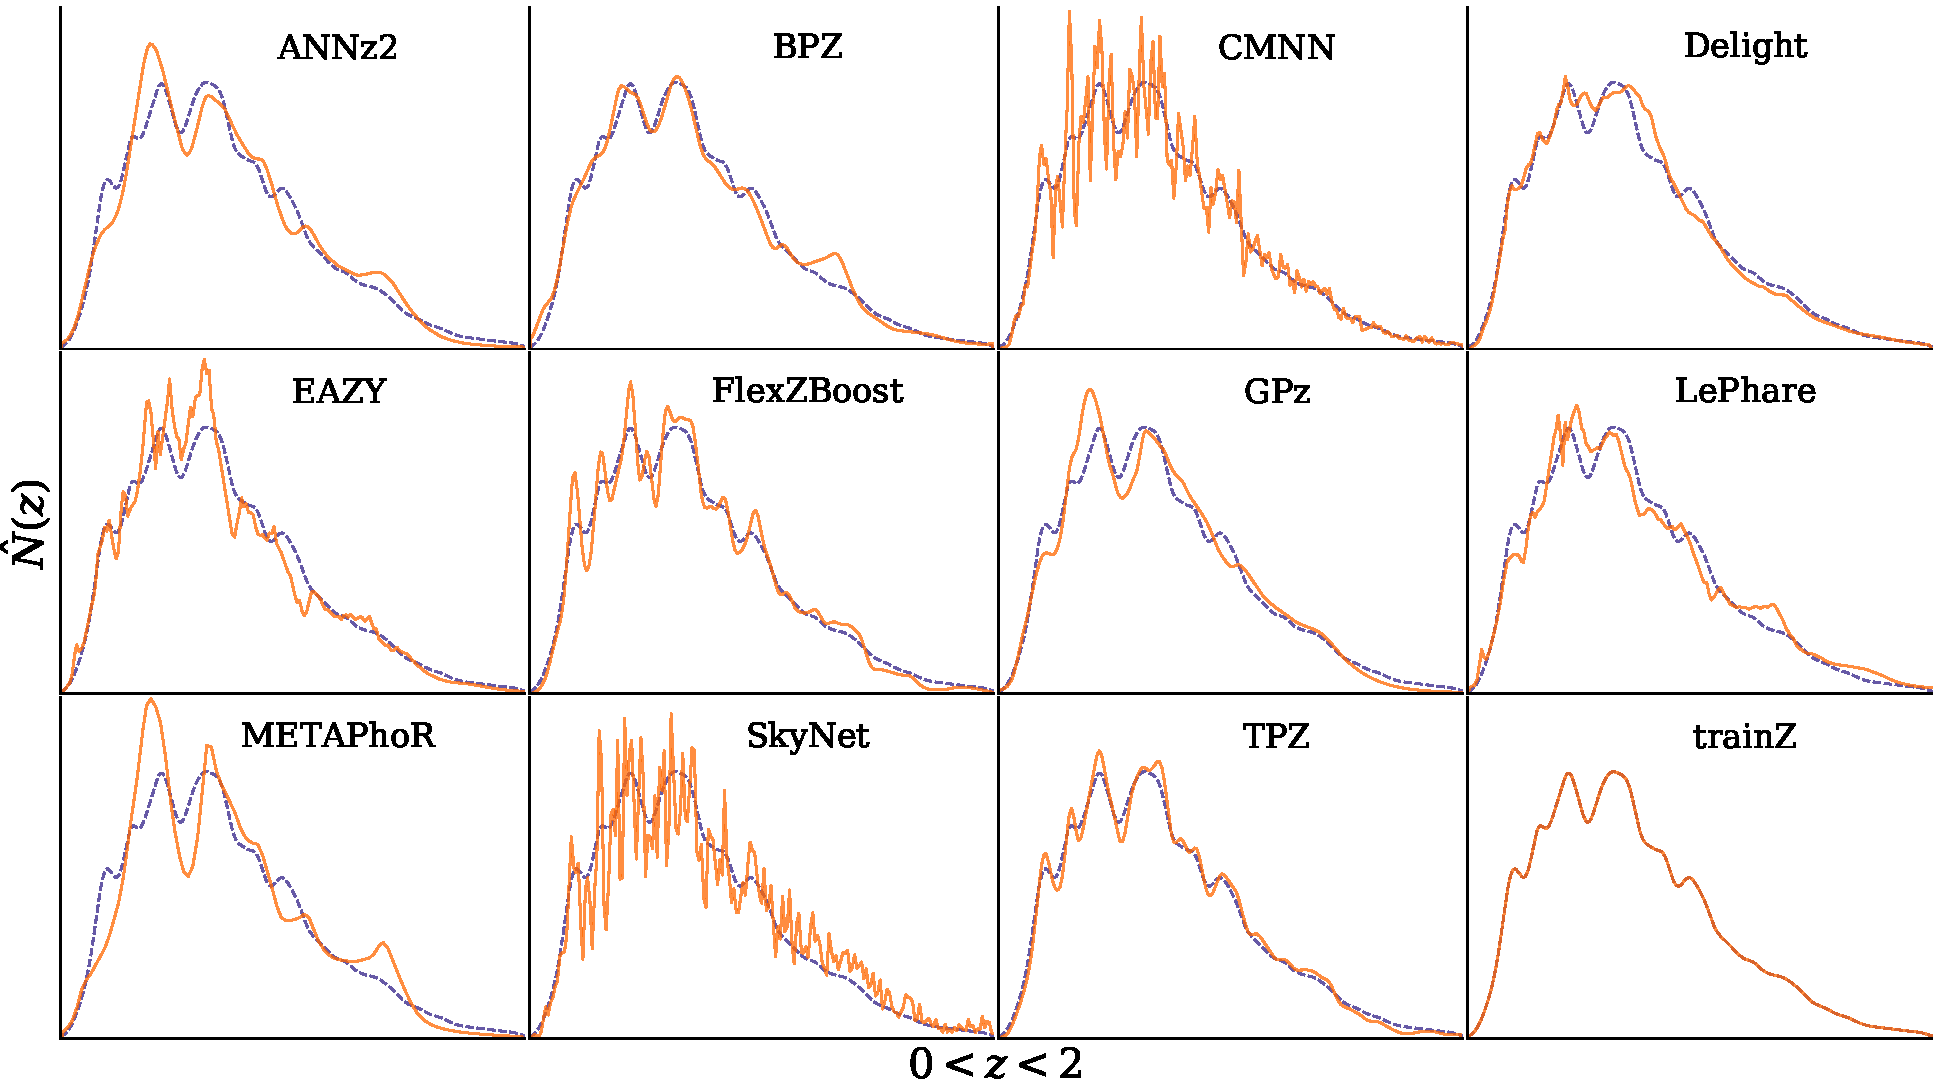
\includegraphics[width=\textwidth]{figures/pzdc1/NZsumplot_AIM.pdf}
	\caption[The smoothed stacked estimator $\hat{N}(z)$ of the redshift distribution produced by each code considered in \Chap{pzdc1}]
	{The smoothed stacked estimator $\hat{N}(z)$ of the redshift distribution (orange) produced by each code (panels) compared to the true redshift distribution $\tilde{N}(z)$ (purple dashed).
		Varying levels of agreement are seen among the codes, with the smallest deviations for \cmnn, \flexzboost, \tpz, and \trainz.}
	\figlabel{fig:nz}
	%\aim{Arguably this could also be clarified by showing the true $n'(z)$ once and then differences from it for each cod's stacked estimator\dots}\scc{what if we plot the difference between true and stacked rather than soverposing the two lines? Sam please do not hate me.}
\end{figure*}

Many of the codes, including all the model-fitting approaches and \annz, \gpz, \metaphor, and \skynet\ from the data-driven camp, overestimate the redshift density at $z \sim 1.4$.
This behavior is a consequence of the $4000 \rm{\AA}$ break passing through the gap between the $z$ and $y$ filters, which induces a dramatic rise and fall in the $z - y$ colour as a function of redshift.  
With a dearth of strong spectral features blue-ward of the 4000 \AA\ break in most galaxy SEDs, the degeneracies on either side of the peak in $z - y$ colour tend to broaden the redshift PDFs near $z \sim 1.4$, which can lead to the ``bump'' seen in the stacked $\hat{N}(z)$ estimate.

% \annz, \gpz, and \metaphor\ show signs of overtraining, estimating enhanced peaks and diminished troughs relative to the training set, an obstacle that may be overcome with adjustment of the implementation.
\annz, \gpz, and \metaphor\ feature exaggerated peaks and troughs relative to the training set, a potential sign of overtraining.
Further investigation on overtraining is needed, if present this is an obstacle that may be overcome with adjustment of the implementation.

As expected, \trainz\ perfectly recovers the true redshift distribution: as the training sample is selected from the same underlying distribution as the test set, the redshift distributions are identical, up to Poisson fluctuations due to the finite number of sample galaxies.
\cmnn\ is also in excellent agreement for similar reasons: with a representative training sample of galaxies spanning the colour-space, the sum of the colour-matched neighbour redshifts should return the true redshift distribution.
\flexzboost\ and \tpz\ also perform superb recovery of the true redshift distribution, with only a slight deviation at $z \sim 1.4$.
Our metrics, however, cannot discern whether these four approaches, as well as \delight, are spared the $z \sim 1.4$ degeneracy in $\hat{N}(z)$ because they have more effectively used information in the data or if the impact is simply washed out by the stacked estimator's effective average over the test set galaxy sample.
See Appendix~\ref{sec:pointmetrics_results} for further discussion of the $z \sim 1.4$ issue.

\Fig{fig:nz_stats} shows the quantitative Kolmogorov-Smirnoff (KS), Cramer-Von Mises (CvM), and Anderson Darling (AD) test statistics for each of the codes for the $\hat{N}(z)$ based measures.
%The horizontal lines show the result of a bootstrap resampling of the training set using $44 404$ samples for \trainz, representing a conservative statistical error estimate assuming our modest-sized representative training set of galaxies, as mentioned in Section~\ref{pzdc1:sect:sec:pitqq}.
%The AD bootstrap statistic is elevated due to its sensitivity to the tails of distributions.
%\red{Can p-values be supplied for each statistic? The statistics themselves are difficult to interpret, other than ``lower is better'' (no, p-values are very difficult to compute for non-uniform distributions)}
The stacked estimators of the redshift distribution for \cmnn\ and \trainz\ best estimate $\tilde{N}(z)$ under these metrics, whereas \eazy, \lephare, \metaphor, and \skynet\ underperform; \bpz, \gpz, and \tpz\ are within a factor of two of the conservative \trainz\ bootstrap-based limit for all statistics.
It is unsurprising that \cmnn\ scores well, as with a nearly complete and representative training set choosing neighbouring points in color/magnitude space to construct an estimator should lead to excellent agreement in the final $\hat{N}(z)$.

\begin{figure*}
	\centering
	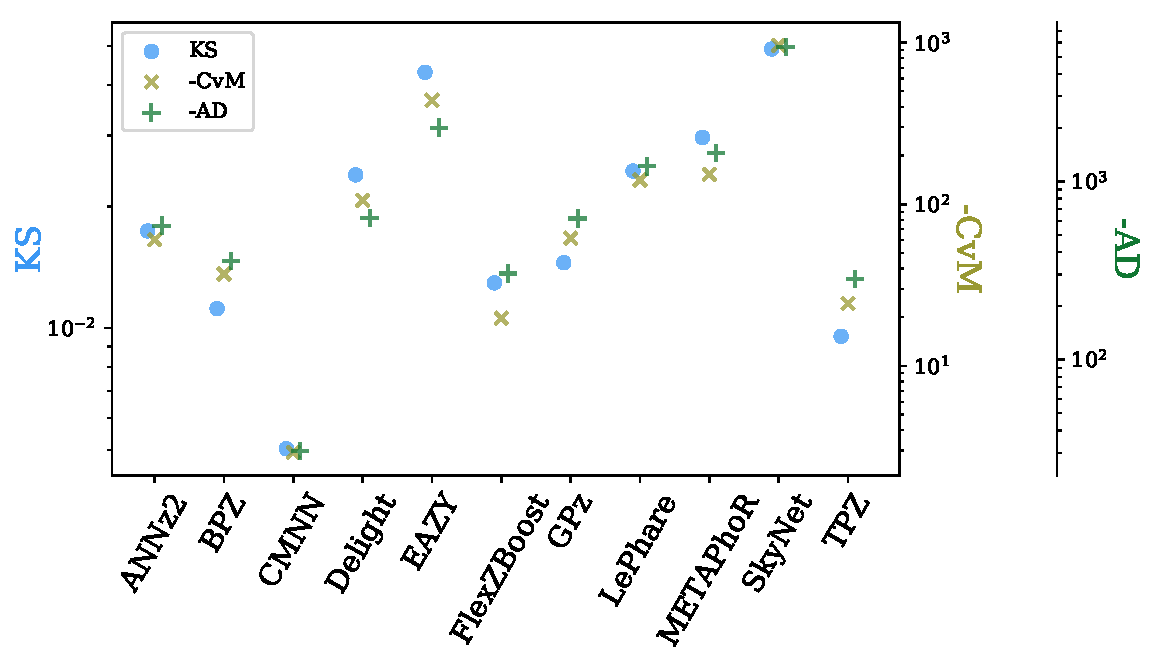
\includegraphics[width=0.98\textwidth]{figures/pzdc1/KSvsCvMvsAD_Nz.pdf}
	\caption[The Kolmogorov-Smirnoff, Cramer-von Mises, and Anderson-Darling statistics for the $\hat{N}(z)$ distributions of each code considered in \Chap{pzdc1}]
	{The Kolmogorov-Smirnoff (KS, blue $\bullet$), Cramer-von Mises (CvM, yellow $\times$), and Anderson-Darling (AD, green $+$) statistics for the $\hat{N}(z)$ distributions.
		We make the reassuring observation that these related statistics do not disagree significantly with one another.
		\cmnn\ outperforms the control case, \trainz, and several codes are within a factor of two of this conservative idealized limit.
		\skynet\ scores poorly due to an overall bias in its redshift predictions.}
	\figlabel{fig:nz_stats}
\end{figure*}

It is, however, surprising that \tpz\ does well on $\hat{N}(z)$ given its poor performance on the ensemble \pzpdf s, especially knowing that \tpz\ was optimized for \pzpdf\ ensemble metrics rather than the stacked estimator of the redshift distribution.
A possible explanation is the choice of smoothing parameter chosen during validation, which affects \pzpdf\ widths as well as overall redshift bias and could be modified to improve performance under the \pzpdf\ metrics.
Evaluation of Supplemental Metrics of \Pzpdf s
The first three moments of the stacked $\hat{N}(z)$ distribution relative to the empirical estimate of the truth distribution are given in \Tab{tab:moments}.
Accuracy of the moments varies widely between codes, raising concerns about the propagation to cosmological analyses.
%\red{[mention that we are calculating moments for the entire sample, will look at fiducial tomographic bins in a follow-up paper (unless group and reviewers realy think we should include in this paper.]}
%\red{FlexZBoost has some of the best $n(z)$ statistics, but the moments are not good.  Why is this?  Is it the over/underprediction of the high redshift part of the distribution?  Discuss this after talking with Rafael.}

\begin{table}
	\begin{center}
		\setlength{\tabcolsep}{2pt}
		\caption[Moments of the stacked estimator $\hat{N}(z)$ of the redshift distribution for the codes of \Chap{pzdc1}]
		{Moments of the stacked estimator $\hat{N}(z)$ of the redshift distribution.
			Most of the codes considered recover the moments of $\tilde{N}(z)$}
		\tablabel{tab:moments}
		\begin{tabular}{lccc}
			\hline
			\hline
			\multicolumn{4}{l}{Moments of $\hat{N}(z)$} \\
			\hline
			Estimator  & mean       & variance    & skewness \\
			Empirical ``truth'' & 0.701 & 0.630 & 0.671  \\
			\hline
			\annz       & 0.702      & 0.625      & 0.653    \\
			\bpz        & 0.699      & 0.629      & 0.671    \\
			\delight    & 0.692      & 0.609      & 0.638    \\
			\eazy       & 0.681      & 0.595      & 0.619    \\
			\flexzboost & 0.694      & 0.610      & 0.631    \\
			\gpz        & 0.696      & 0.615      & 0.639    \\
			\lephare    & 0.718      & 0.668      & 0.741    \\
			\metaphor   & 0.705      & 0.628      & 0.657    \\
			\cmnn       & 0.701      & 0.628      & 0.667    \\
			\skynet     & 0.743      & 0.708      & 0.797    \\
			\tpz        & 0.700      & 0.619      & 0.643    \\
			\hline
			\trainz	    & 0.699 		 & 0.627 	    & 0.666 \\
		\end{tabular}
	\end{center}
\end{table}


We calculated the first three moments of the stacked $\hat{N}(z)$ distribution of all galaxies and compared it to the moments of the true redshift distribution.  
\Tab{tab:moments} shows the residuals of the moments for all codes.  
Accuracy of the moments varies widely between codes, raising concerns about the propagation to cosmological analyses.  
The DESC SRD \citep{the_lsst_dark_energy_science_collaboration_lsst_2018} lists stringent requirements on how well the mean and variance of tomographic redshift bins must be known for each of the main DESC science cases.  
We indicate the Year 10 (Y10) requirements assuming our true mean redshift of $z=0.701$ as dashed lines.  
In this study with representative training data, \annz, \cmnn, \tpz, and our pathological \trainz\ estimator meet the Y10 requirement on the mean redshift.  Only \annz, \cmnn, and \trainz\ meet both requirements.  
One should be concerned that many codes fail to meet this ambitious limit under perfect prior information because all codes are anticipated to do no better under realistically imperfect prior information, and indicates that additional calibration to remove these systematic offsets \citep[e.~g.~][]{newman_calibrating_2008} will likely be necessary in order to meet these stringent goals.


\skynet\ exhibits redshift bias in \Fig{fig:nz} and is a clear outlier in the first moment of $\hat{N}(z)$ in \Tab{tab:moments}.
The \skynet\ algorithm employs a random subsampling of the training set without testing that the subset is representative of the full population, and the implementation used here does not upweight rarer low- and high-redshift galaxies, as in \citet{bonnett_using_2015}, suggesting a possible cause that may be addressed in future work.

\subsection{\Pz\ point estimation and metrics}
%\appendices{\Pz\ point estimation and metrics}
\label{sec:allpointmetrics}

While this work assumes that science applications value the information of the full \pzpdf, we present conventional metrics of \pz\ point estimates as a quick and dirty visual diagnostic tool and to facilitate direct comparisons to historical studies.

\subsubsection{Reduction of \pzpdf s to point estimates}
\label{sec:pointest}

Though we acknowledge that many of the codes can also return a native \pz\ point estimate, we put all codes on equal footing by considering two generic \pz\ point estimators, the mode $z_{PEAK}$ and main-peak-mean $z_{WEIGHT}$ \citep{dahlen_critical_2013}, a weighted mean within the bounds of the main peak, as identified by the roots of $p(z) - 0.05 \times z_{PEAK}$.
Though $z_{WEIGHT}$ neglects information in a secondary peak of e.~g.~ a bimodal distribution, it avoids the pitfall of reducing the \pzpdf\ to a redshift between peaks where there is low probability.

\subsubsection{Metrics of \pz\ point estimates}
\label{sec:pointmetrics}

We calculate the commonly used point estimate metrics of the overall intrinsic scatter, bias, and catastrophic outlier rate, defined in terms of the standard error $e_{z} \equiv (z_{PEAK} - z_{\rm true}) / (1 + z_{\rm true})$.
Because the standard deviation of the \pz\ residuals is sensitive to outliers, we define the scatter in terms of the Interquartile Range (IQR), the difference between the 75th and 25th percentiles of the distribution of $e_{z}$, imposing the scaling $\sigma_{\rm IQR} = \rm{IQR} / 1.349$ to ensure that the area within $\sigma_{\rm IQR}$ is the same as that within one standard deviation from a standard Normal distribution.
We also resist the effect of catastrophic outliers by defining the bias $b_{z}$ as the median rather than mean value of $e_{z}$.
The catastrophic outlier rate $f_{\rm out}$ is defined as the fraction of galaxies with $e_{z}$ greater than $\max(3 \sigma_{\rm IQR}, 0.06)$.
For reference, Section 3.8 of the \lsst\ Science Book \citep{lsst_science_collaboration_lsst_2009} uses the standard definitions of these parameters, given in Table~\ref{intro:tab:tab:lsstsrd}.
%\begin{itemize}
%	\item RMS scatter $\sigma < 0.02 (1 + z_{\rm true})$
%	%\scc{actually the SB reports in page 75 that the goal of 0.02 is for the RMS of $\frac{\sigma_{z}}{(1+z)}$ while we are usEvaluation of Supplemental Metrics of \Pzpdf sing IQR}
%	\item bias $b_{z} < 0.003$ %\scc{in page 518 of the SB is clearly reported that the mean is expected to be less than 0.003 in our case we have defined as bias the median and not the mean }
%	\item catastrophic outlier rate $f_{\rm out} < 10\%$ %\scc{clearly the number of outliers since are defined above $3\sigma$ strictly depends on the sigma definition, in the science book it seems to refer to the RMS of the $e_z$ distribution even ef it could be the standard deviation, but again I don't think it refers to IQR, therefore we could not consider exactly this numbers as reference.}
%	%\red{I am going off of conversations with Zeljko and how we {\it actually} computed the metrics in the Science Book (I have the scripts).  You are correct that several of these are slightly different than actually stated in the Science Book, or where the Science Book does not use very precise language as to what was done to compute the RMS or define the bias.  We can also cut out those specifics, or maybe say Ivezic private communication, maybe?  Also $\sigma_{z}$ defined in terms of IQR is exactly equivalent to the standard deviation when scaled by 1.349 for a Gaussian distribution, so the numbers are appropriate to cite in this context.  IQR is just a more robust way of calculating sigma for a distribution with outliers.--SJS }
%	%\scc{I am very sorry I am not saying that IQR is not fine, I want to keep the IQR my concerns are related to the notation and the \textit{reader understanding}, if I wrote $\sigma$ somewhere in a table the reader will understand for sure that is the traditional standard deviation (a lot of people skips the indicators definition for the \textit{obvious} ones), I am suggesting to replace the notation $\sigma$ with the notation $\sigma_{IQR}$ (or something like this) to avoid any confusion, and also to change from $bias$ to $median$ for the same reason. I agree that say Ivezic private communication could be better.}
%	.
%\end{itemize}

\subsubsection{Comparison of \pz\ point estimate metrics}
\label{sec:pointmetrics_results}

\Fig{fig:pz_pointestimates_peak} and \Fig{fig:pz_pointestimates_weight} show the $z_{PEAK}$ and $z_{WEIGHT}$ point estimates, respectively, versus true redshift for all codes.
Point density is shown with mixed contours to emphasize that most of the galaxies do fall close to the $\hat{z} = z_{true}$ line, while points trace the details of the catastrophic outlier populations.

\begin{figure*}
	\centering
	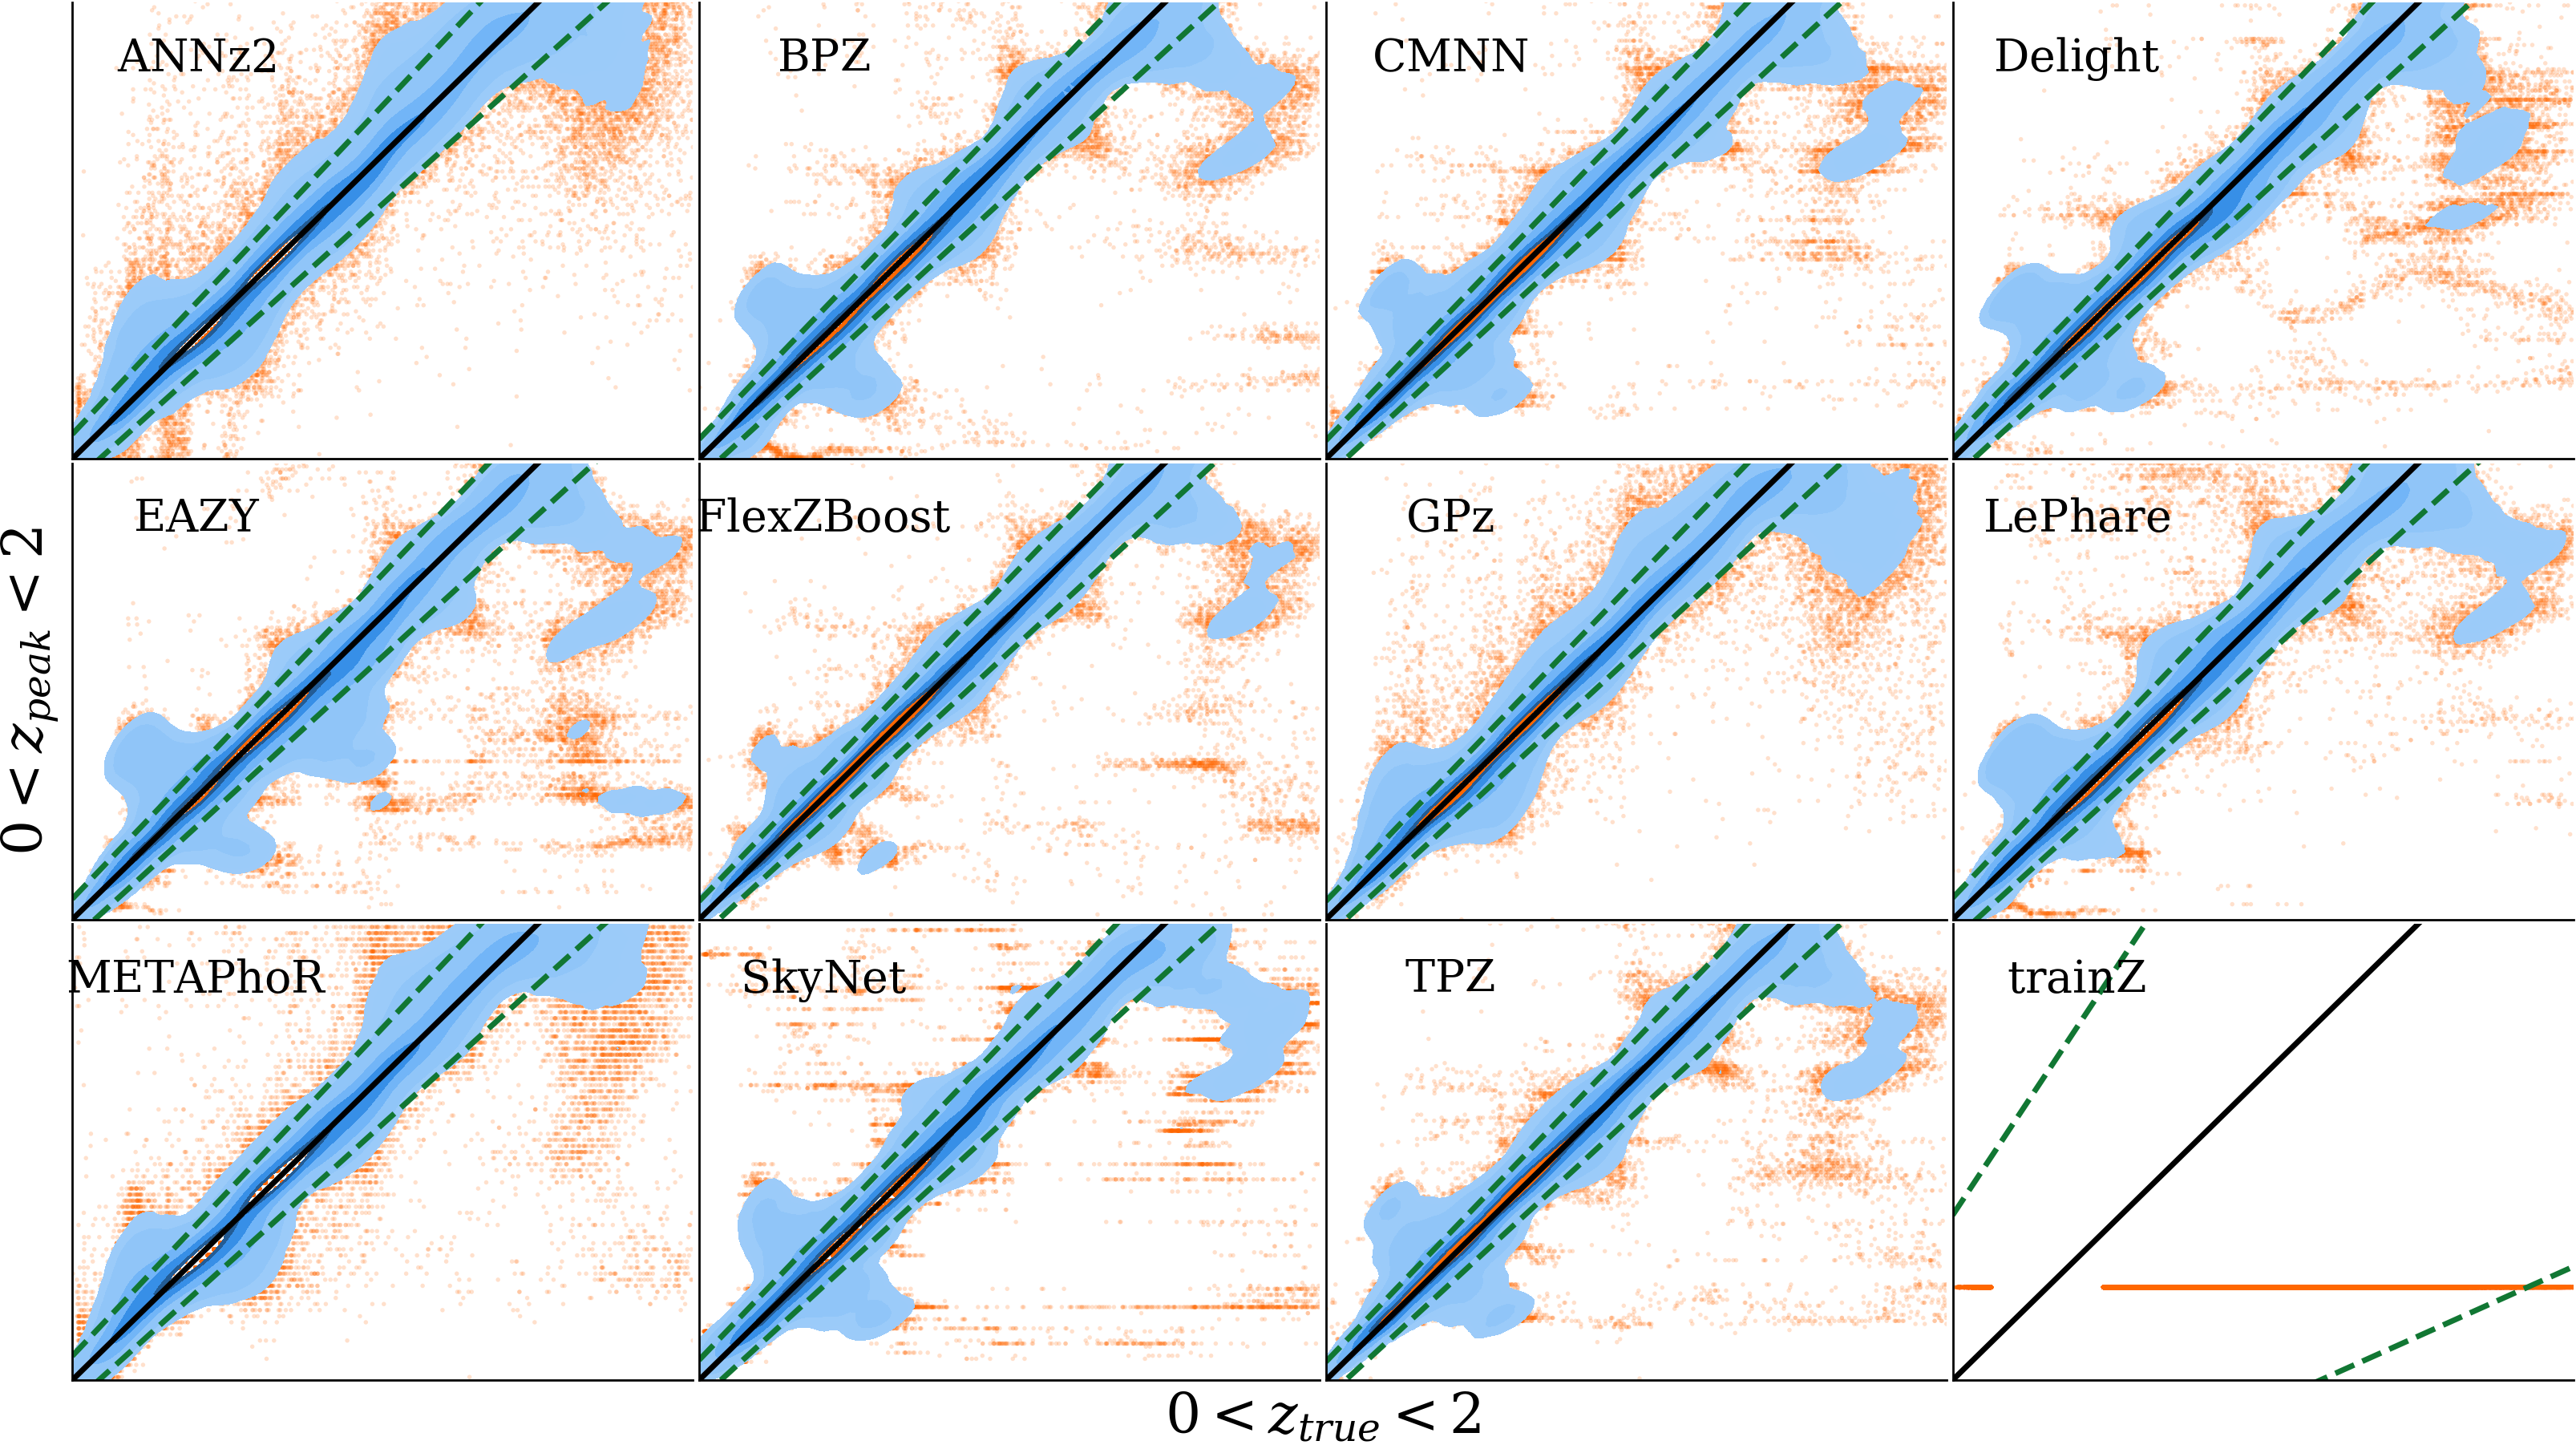
\includegraphics[width=0.74\textwidth]{figures/pzdc1/ZPEAK_AIM.png}
	\caption[The density of \pz\ point estimates reduced from the \pzpdf s via the mode for the codes considered in \Chap{pzdc1}]
	{The density of \pz\ point estimates (blue contours) reduced from the \pzpdf s with outliers (orange) beyond the outlier cutoff (green dashed lines) via the mode.
		The \trainz\ estimator (lower right sub-panels) has a shared $z_{PEAK}$ for the entire test set galaxy sample.
		%	\aim{Overhaul these plots for readability.}
	}
	\figlabel{fig:pz_pointestimates_peak}
\end{figure*}

\begin{figure*}
	\centering
	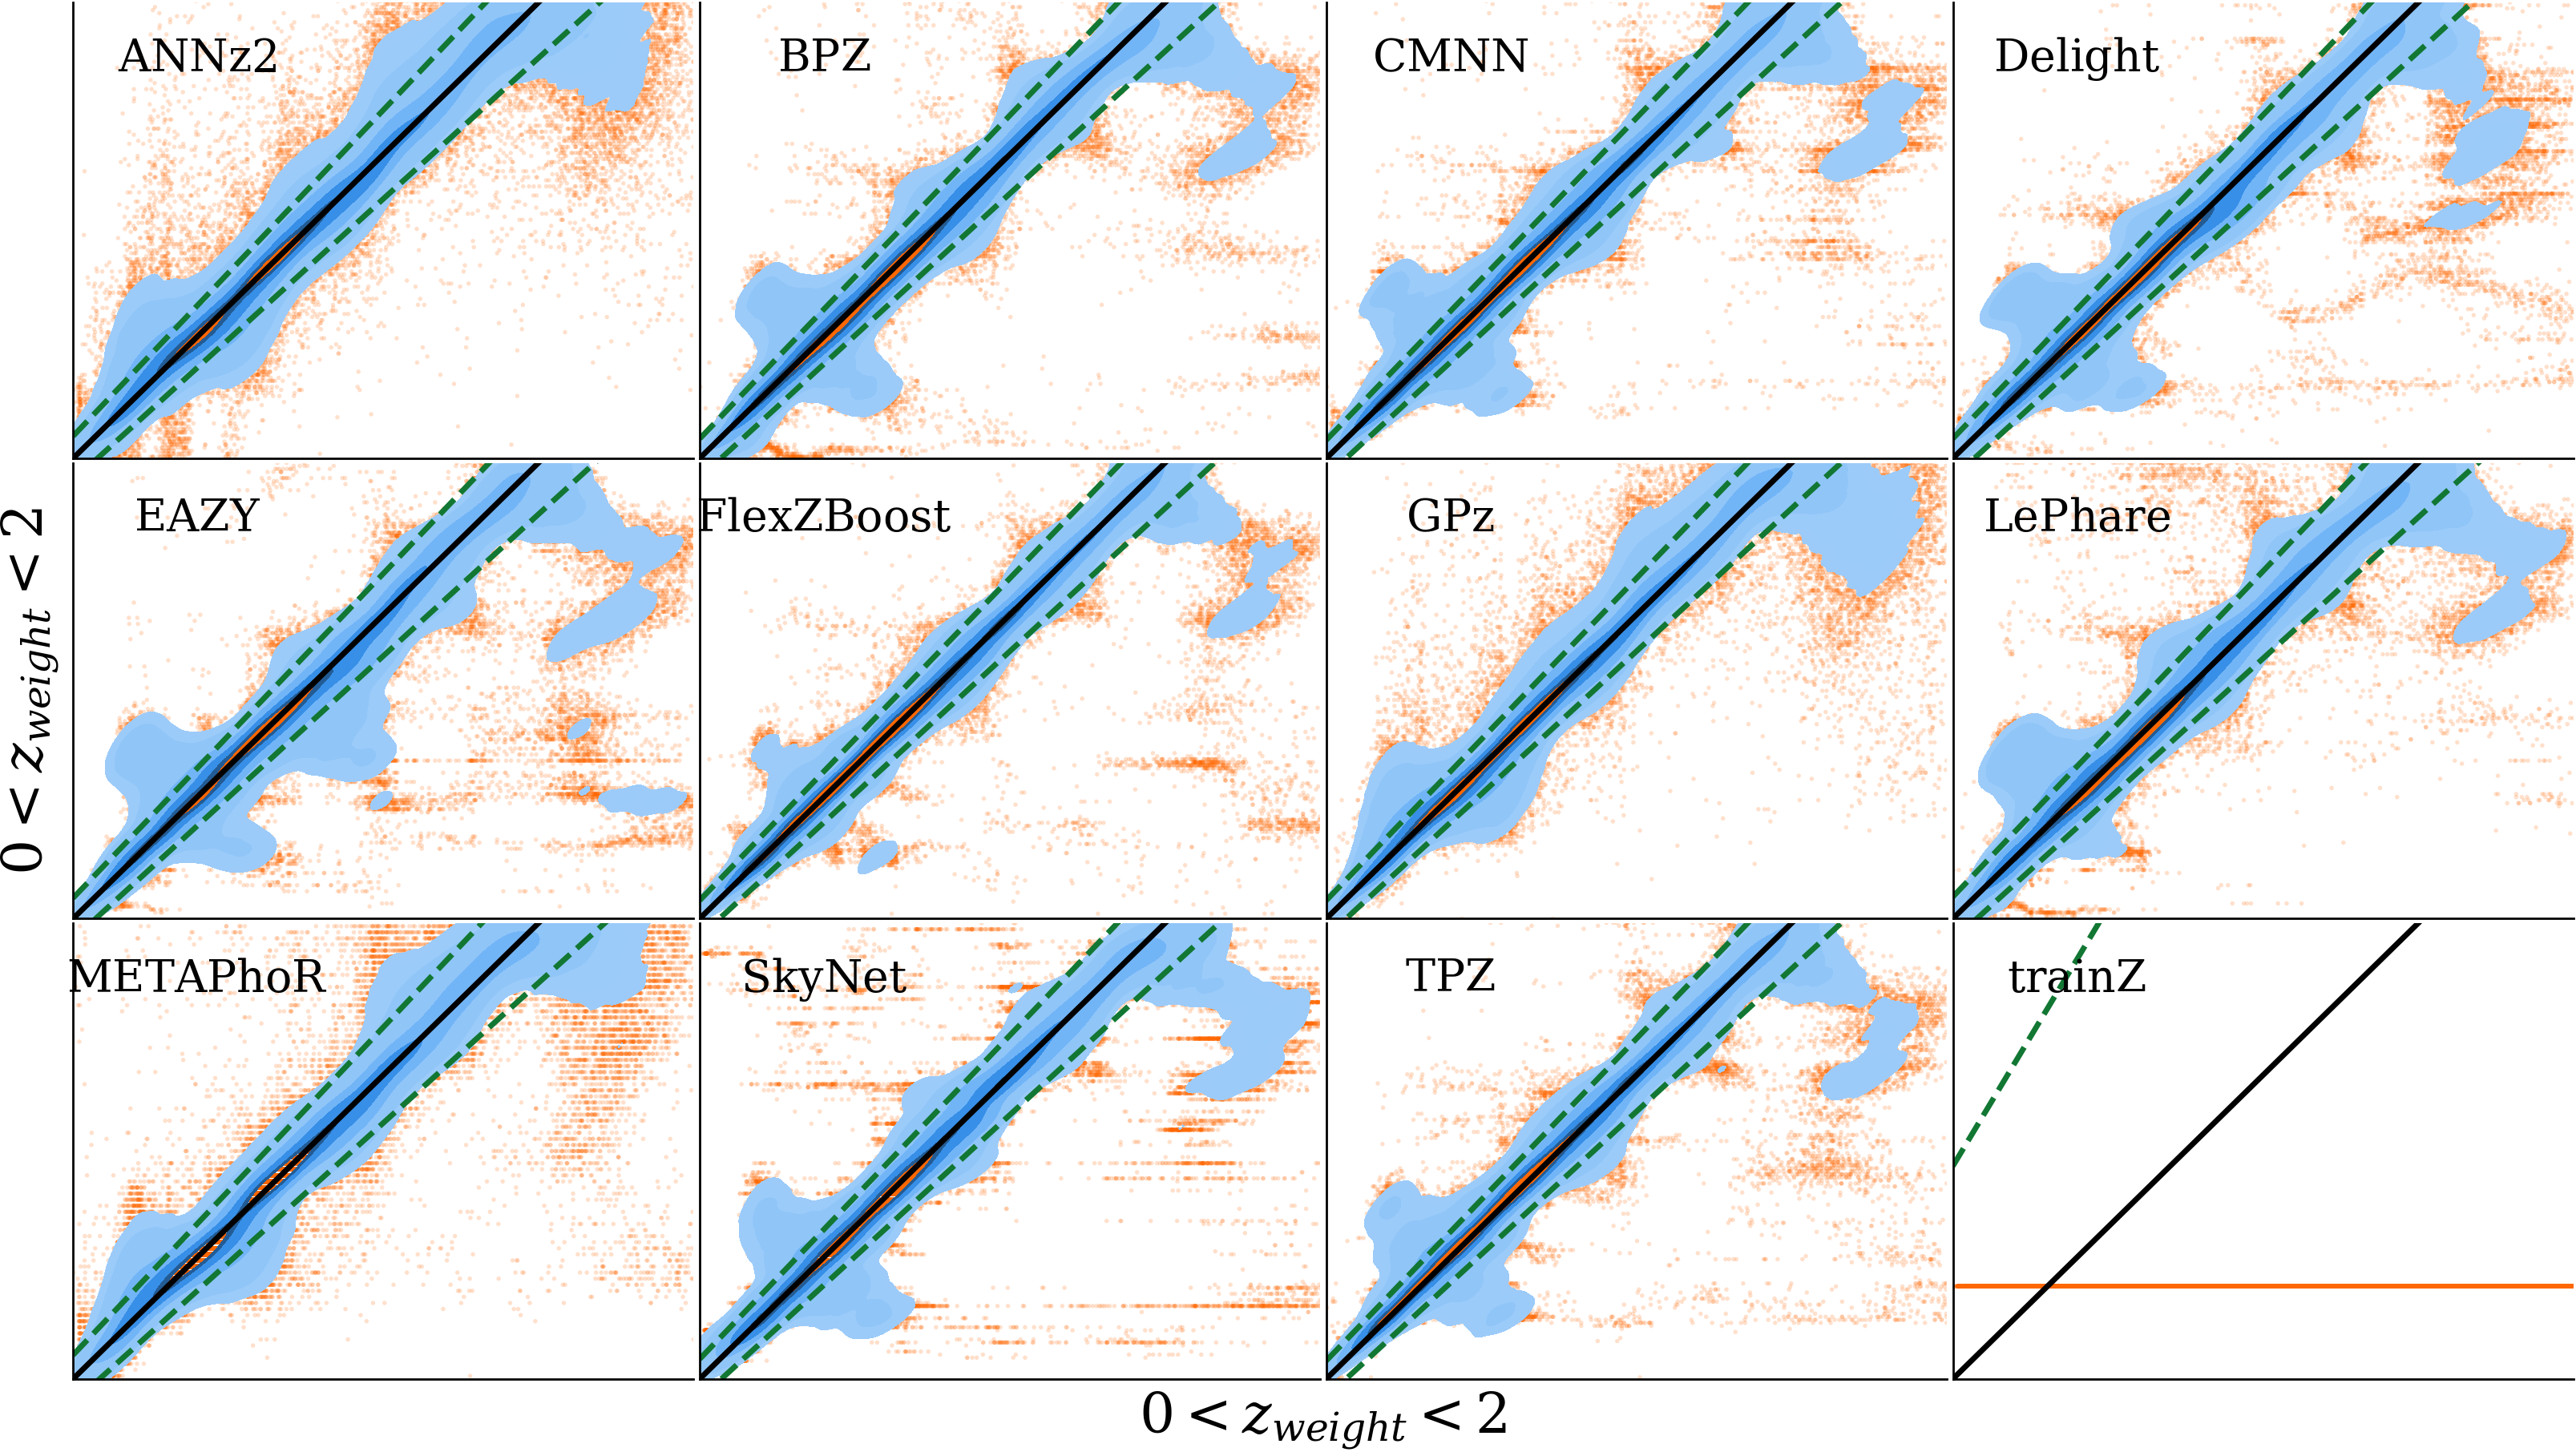
\includegraphics[width=0.74\textwidth]{figures/pzdc1/ZWEIGHT_AIM.png}
	\caption[The density of \pz\ point estimates reduced from the \pzpdf s via the main-peak-mean for the codes considered in \Chap{pzdc1}]
	{The density of \pz\ point estimates (blue contours) reduced from the \pzpdf s with outliers (orange) beyond the outlier cutoff (green dashed lines) via the main-peak-mean.
		The \trainz\ estimator (lower right sub-panels) has a shared $z_{WEIGHT}$ for the entire test set galaxy sample.
		%	\aim{Overhaul these plots for readability.}
	}
	\figlabel{fig:pz_pointestimates_weight}
\end{figure*}

The finite grid spacing of the \pzpdf s induces some discretization in $z_{PEAK}$.%, particularly for \skynet.
% \aim{TODO: paopagate to GitHub}
The features perpendicular to the $\hat{z} = z_{true}$ line are due to the $4000 \rm{\AA}$ break passing through the gaps between adjacent filters, most notably at $z \sim 0.4$ between the $g$ and $r$ filters and at $z \sim 1.4$ between the $z$ and $y$ filters.  
All codes show some level of concentrated catastrophic outliers, often due to degenerate redshift solutions for a single area of color space.  
In the presence of genuine ambiguities in the colour-space-to-redshift mapping, the reduction of information down to a single number that is the point estimate redshift fails to adequately capture the more complex nature of the multimodal redshift matching: 
using the mode selects the highest peak while ignoring posterior probability in lower valued redshift peaks, while measuring the mean of a multimodal PDF often results in a value lying at a redshift between the peaks, removed from either/any of the most likely redshift solutions.  
Thus even the strongest codes feature populations far from the $\hat{z} = z_{true}$ line representing a genuine degeneracy in the space of colours and redshifts.
% and logically are more prominent for template-based codes
%Even the strongest codes feature populations far from the $z_{phot} = z_{spec}$ line representing a degeneracy in the space of colours and redshifts.
% While use of the full information available via $p(z)$ mitigates their impact, a full understanding of the outlier population is critical for LSST science, particularly in tomographic applications.
%\red{I forget what exactly I was trying to say here, if someone else wants to take a crack at this it might be helpful --SJS}
%\scc{may be worth to say that the usage of further bands could mitigate this effect by removing the degeneration  usually induced from emission lines moving across different filters?}

\begin{table*}
	\begin{center}
		\caption[\Pz\ point estimate summary statistics for the codes of \Chap{pzdc1}]
		{\Pz\ point estimate summary statistics}
		\tablabel{tab:pointestimates}
		\begin{tabular}{lcccccc}
			\hline
			\hline
			&            & $z_{PEAK}$  &          &  & $z_{WEIGHT}$          &\\
			\hline
			\Pz\ Code       & $\frac{\sigma_{IQR}}{(1+z)}$ & median  & \multicolumn{1}{|p{0.75cm}|}{\centering outlier \\fraction} & $\frac{\sigma_{IQR}}{(1+z)}$ & median & \multicolumn{1}{|p{0.75cm}|}{\centering outlier \\fraction}\\
			\hline
			\annz     & 0.0270  &  0.00063  & 0.044      & 0.0244  &  0.000307  & 0.047  \\
			\bpz       & 0.0215  & -0.00175  & 0.035      & 0.0215  & -0.002005  & 0.032 \\
			\delight   & 0.0212  & -0.00185  & 0.038      & 0.0216  & -0.002158  & 0.038 \\
			\eazy      & 0.0225  & -0.00218  & 0.034      & 0.0226  & -0.003765  & 0.029 \\
			\flexzboost& 0.0154  & -0.00027  & 0.020      & 0.0148  & -0.000211  & 0.017 \\
			\gpz       & 0.0197  & -0.00000  & 0.052      & 0.0195  &  0.000113  & 0.051 \\
			\lephare   & 0.0236  & -0.00161  & 0.058      & 0.0239  & -0.002007  & 0.056 \\
			\metaphor  & 0.0264  &  0.00000  & 0.037      & 0.0262  &  0.001333  & 0.048 \\
			\cmnn        & 0.0184  & -0.00132  & 0.035      & 0.0170  & -0.001049  & 0.034 \\
			\skynet    & 0.0219  & -0.00167  & 0.036      & 0.0218  &  0.000174  & 0.037 \\
			\tpz       & 0.0161  &  0.00309  & 0.033      & 0.0166  &  0.003048  & 0.031 \\
			\hline
			\trainz	   & 0.1808  &  -0.2086  & 0.000	  & 0.2335  & 0.022135  & 0.000\\
		\end{tabular}
	\end{center}
\end{table*}

The intrinsic scatter, bias, and catastrophic outlier rate are given in \Tab{tab:pointestimates}.
Perhaps unsurprisingly, performance under these metrics largely tracks that of the metrics of Section~\ref{pzdc1:sect:sec:metrics} of the \pzpdf s from which the point estimates were derived.
All twelve codes perform at or near the goals of the \lsst\ Science Requirements Document\footnote{available at: \url{http://ls.st/srd}} and \citet{graham_photometric_2018}, which is encouraging if not unexpected for $i < 25.3$.
% But, it is still an encouraging sign, given an updated mock galaxy simulation and the expanded set of	 photo-$z$ codes tested.
%\red{maybe say consistent with expectations, and a reference to Melissa's paper in here?  What else to say about nearly meeting point goals?}

%\section{Chapter acknowledgements}
%
%I express gratitude to
%[helpful people here]
%for their contributions to this work.
